\documentclass{asaproc}
%\documentclass{article}
\usepackage{amssymb,amsmath,amsthm}
\usepackage{graphicx}
%\usepackage[ruled,linesnumbered]{algorithm2e}
\usepackage[caption = false]{subfig}
\usepackage{float}

%\usepackage{times}
%If you have times installed on your system, please
%uncomment the line above

%For figures and tables to stretch across two columns
%use \begin{figure*} \end{figure*} and
%\begin{table*}\end{table*}
% please place figures & tables as close as possible
% to text references

% Commands
\newcommand{\sq}{\sigma^2}
\newcommand{\tq}{\tau^2}
\newcommand{\laq}{\lambda^2}
\newcommand{\bh}{\hat{\beta}}
\newcommand{\Sh}{\hat{\Sigma}}

% Figures Path
\graphicspath{{./fig/}}

\title{Defending Against Adversarial Attacks}

%input all authors' names

\author{Brett Gohre, Rene Gutierrez \& Keller Jordan \\ }

%input affiliations

%{USDA Forest Service Forest Products Laboratory}

\begin{document}

\maketitle


\begin{abstract}
	
Adversarial attacks have been a growing concern as the success of Neural Networks increases. Of particular interest, are attacks that can devised without knowing the particular model used, but only the data distribution, the so called Black Box attacks. In this project we test several ideas to fend off Black Box attacks, Random Compression Matrices, Multi-task Training, Detection using Reconstruction Error and Capsule Networks.
	
\begin{keywords}
Adversarial Examples, Black-Box Attacks, Random Projection Matrix, Multi-Task Training, Reconstruction Error, Capsule Networks, Convolutional Neural Networks.
\end{keywords}
\end{abstract}


\section{Introduction}

There is an increasing concern that Neural Networks are very susceptible to Black Box Adversarial Attacks, with implications that go from identity theft, as in biometrics recognition to safety in the self-driving car industry. So it is of the utmost importance to try to create defenses against such attacks, or at the very least study their characteristics. Here we try several alternatives with varying degrees of success, however even in failure, new insights are gained in exploration.

\section{Random Projection Matrices}

\subsection*{Idea}

Random compression matrices have been found to be able to perform dimensionality reduction exploiting the input data structure, in particular when the data could belong to a manifold. We can make further use of this in two ways, first the dimensionality reduction can help create smaller models that could help robustness. Furthermore, the random nature of the matrix can transform the attack and make it less or not powerful at all.

\subsection*{Method}

For this idea we worked with the MNIST dataset. First created 2 sets of adversarial examples based on different architectures. The first set was based on Logistic Regression and consists of 758 adversarial images. The second one was based on a Convolutional Neural Network optimized to 95\% accuracy in the validation set, and had 440 adversarial images. Then we tried to attack these architectures plus a Random Compression Matrix architecture, a Random Expansion Matrix and 2 CNN optimized to 90\% and 99\% accuracy.

The Random Projection architectures where basically a Logistic Regression for which a Random Projection Matrix $ \Phi $ is applied to the input $ x $, but remains fixed through training. The idea was that since adversarial attacks are based on small perturbations $ \epsilon $ to the input, then when applying the random matrix the perturbation would be rendered meaningless, that is $ \Phi \epsilon $ would not be able to attack as effectively. Furthermore, since the attacker would not know $ \Phi $, it would not be able to train attacks specific to it. In this way our random projection matrix can be thought as some kind of code.

\begin{figure}[h!]
	\centering
	\caption{\enspace Examples of the Adversarial Attacks created under the 2 Architechtures. The top row shows the attacks created with the Logistic Regression, while the bottom was created using a CNN.}
	\subfloat[Adversarial Attack for 3]{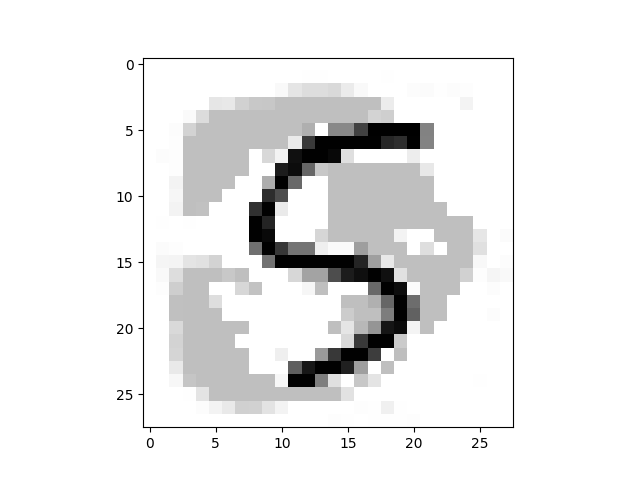
\includegraphics[width=0.45\linewidth]{advImg.png}} 
	\subfloat[Noise  ]{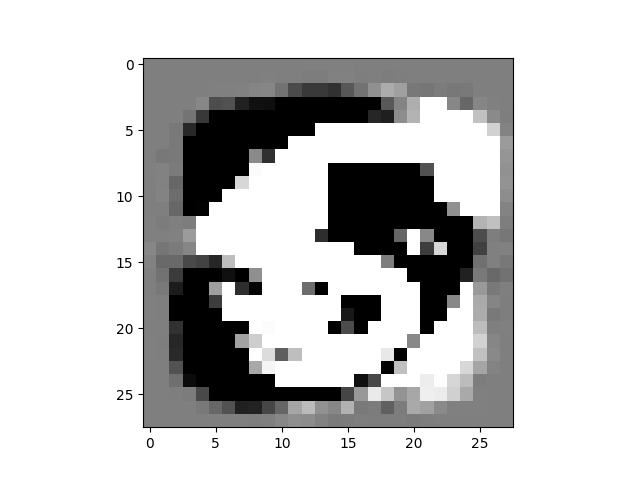
\includegraphics[width=0.45\linewidth]{advNoi.png}}   \\
	\subfloat[Adversarial Attack for 3]{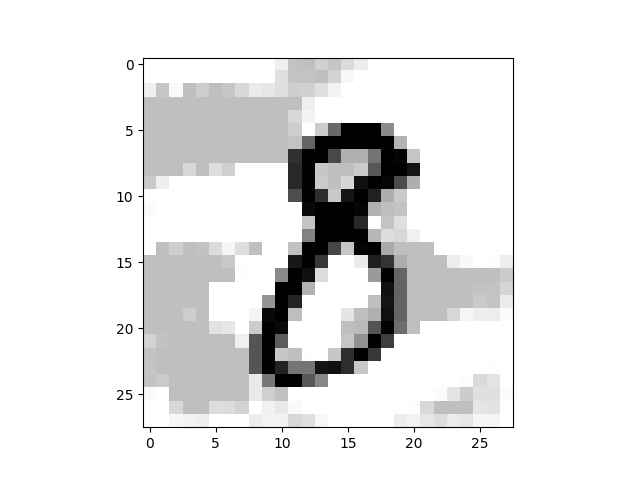
\includegraphics[width=0.45\linewidth]{advImgCnn.png}} 
	\subfloat[Noise  ]{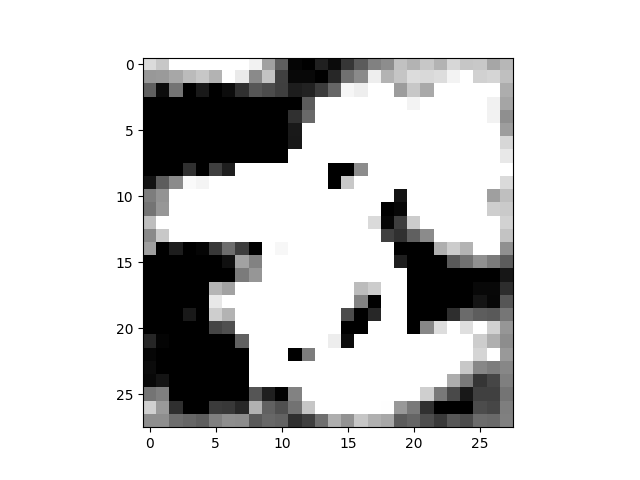
\includegraphics[width=0.45\linewidth]{advNoiCnn.png}}   \\
	\label{fig1}
\end{figure}


\subsection*{Results}

\begin{table*}
	\caption{\enspace Accuracy for the 5 different methods, using the test set and the adversarial examples generated by Logistic Regression and CNN architectures.}
	\label{tab1}
	\begin{tabular*}{\hsize}{@{\extracolsep{\fill}}cccc}
		\hline
		\\[-7pt]
		\multicolumn{1}{c}{\it Method}                    & 
		\multicolumn{1}{c}{\it Test Set}                  & 
		\multicolumn{1}{c}{\it Logistic Arch Adversarial} & 
		\multicolumn{1}{c}{\it CNN Arch Adversarial}      \\
		\hline
		\\[-5pt]
		Logistic Regression      & 92.00\% & 0.00\%  & 3.41\%  \\
		CNN 90\%                 & 89.82\% & 8.71\%  & 5.23\%  \\
		CNN 95\%                 & 94.64\% & 9.50\%  & 9.50\%  \\
		CNN 99\%                 & 98.63\% & 60.95\% & 11.36\% \\
		Compression Logistic to 196 dim & 89.56\% & 0.00\%  & 5.00\%  \\
		Expansion Logistic to 1960 dim  & 91.07\% & 0.00\%  & 3.64\% 
	\end{tabular*}
\end{table*}

\begin{figure}[h!]
	\centering
	\caption{\enspace Confusion Matrices for the True Target and Predicted Target on the Left and the Adversarial Target and Predicted Target on the Right. The top row shows the results using the a compression matrix, while the bottom row shows the results on an expansion matrix. Both results are for the adversarial examples generated with the Logistic Regression architecturee.}
	\subfloat[Confusion Matrix for True Class]{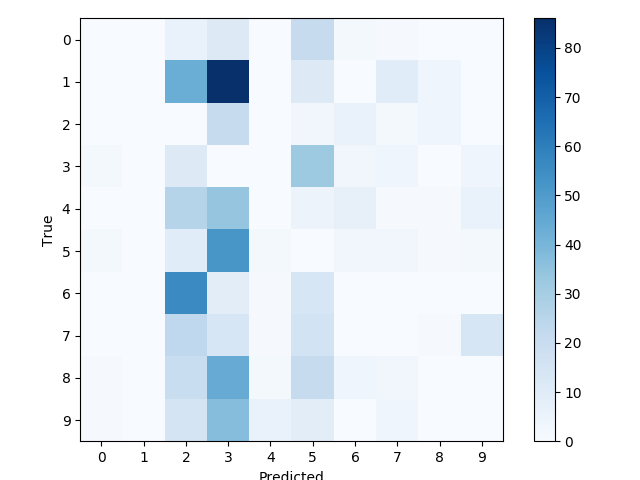
\includegraphics[width=0.5\linewidth]{confussionMatrixAdvTrueCom.png}} 
	\subfloat[Confusion Matrix for Target Class]{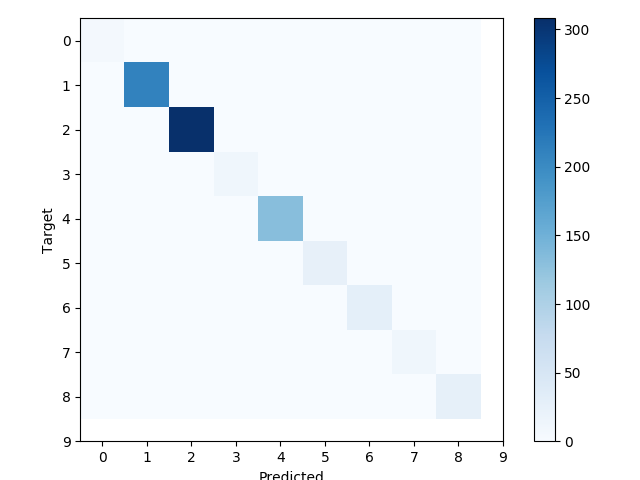
\includegraphics[width=0.5\linewidth]{confussionMatrixAdvTarCom.png}}   \\
	\subfloat[Confusion Matrix for True Class]{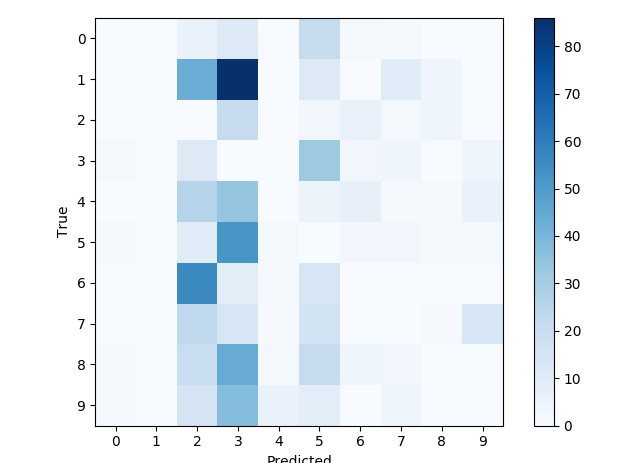
\includegraphics[width=0.5\linewidth]{confussionMatrixAdvTrueExp.png}} 
	\subfloat[Confusion Matrix for Target Class]{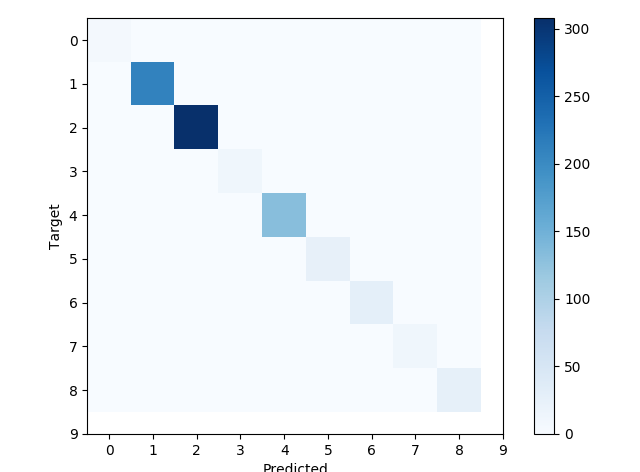
\includegraphics[width=0.5\linewidth]{confussionMatrixAdvTarExp.png}}   \\
	\label{fig2}
\end{figure}

In figure \ref{fig2} we can see the corresponding confusion matrices for the true class on the left and for the adversarial class on the right for the examples generated from the Logistic regression architecture. As we can see the adversarial attacks not only make the expansion and compression defenses fail to predict correctly, but are completely fooled by the examples.

Furthermore, in table \ref{tab1} we can see that the adversarial examples generated by different architectures transfer successfully across architectures. Even fooling completely the randomness induced by the projecting matrices. However it seems that training the CNN to until it achieves higher accuracy provides the best protection, however it still performs poorly and offers little protection for examples generated on the CNN.   

\section*{Multi-task Training with Wingman Distribution}

White box attacks on a separate classifier trained on (approximately) the same data distributions as a black box classifier target. This suggests the data distribution itself contains some weaknesses that can be independently fleshed out with a variety of different types of classifiers. We seek to explore the outcome of training on an additional new classification task with unrelated data. We will train our model to correctly classify the relevant data samples, while simultaneously training the model to correctly classify the irrelevant data samples.

The intuition behind our motivation is that the weight updates may take on a vastly different trajectory than the weight update trajectory of the vanilla case. Bregmann divergences leads to different update rules and they may lead to varying degrees of robustness– if only to attacks based on different divergences. We are curious to find out if multi-task training with the wingman distribution achieve a similar outcomes of defending against attacks.

The assumption is that the attacker does not know what our secret additional domain and task we are training for, and therefore has a worse estimate of the steepest direction toward classifying the input as differently.

\section*{Detection of Adversarial Examples using Reconstruction Error}

\subsection*{Idea}

In the paper introducing Capsule Networks [https://arxiv.org/abs/1710.09829], the capsule network is trained alongside a separate network that attempts to reconstruct the input image from the vector output. The L2 distance between the original image and reconstruction is then added to the loss function and used to train both networks.

When the network is fooled by an adversarial example, the reconstruction produced by the final vector is extremely far from the input image. As a result, it should be possible to use high reconstruction loss as a linear classifier to discern between real inputs and adversarial examples.

\subsection*{Method}

We generated another set of adversarial examples using gradient descent. This time we generated 50,000 for MNIST, we show one of such examples in figure \ref{fig3}. We compute the ROC using the Mean Square Error as a threshold using 50,000 real and 50,000 adversarial examples.

\begin{figure}[h!]
	\centering
	\caption{\enspace EAdversarial Example and Reconstruction. The leftmost image represents the real image, next to it it's corresponding reconstruction. Then we show the adversarial example and finally the corresponding reconstruction on the right.}
	\subfloat[Adversarial and Real Reconstruction]{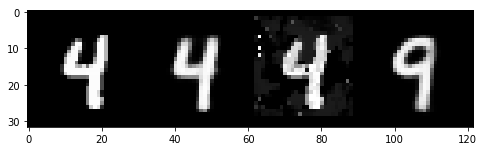
\includegraphics[width=\linewidth]{recon-fig2.png}}
	\label{fig3}
\end{figure}

\subsection*{Results}

As you can see in table the reconstruction error can be used not only to warn against adversarial attacks, but use it also as a linear predictor for adversarial attacks. Finding that setting the threshold for mean square loss at 93 provides a satisfactory defense.

\section*{GD vs ED}

\subsection*{Idea}

Using the square loss results in iterative optimization process as gradient descent, however using the relative entropy loss results in an iterative Exponential gradient update iterative process. In this way we propose using different iterative optimization updates to defend against adversarial attacks generated with the most commonly used gradient descent.

\subsection*{Method}

Again we generate adversarial examples comming from both updating mechanism. 

\subsection*{Results}

As we can see in figure .. using EG instead of GD provides robustness to adversarial attacks.




\bibliographystyle{apalike}
\bibliography{references.bib}


\end{document}




